\chapter{Customization and Tuning: Advanced Lifetime Management Techniques}
\label{chapter:advanced-lifetime-techniques}

\section{Understanding and Tuning the Garbage Collector}

\paragraph{The Collection Schedule and Safe Points}
The garbage collector does not reclaim memory immediately after an object's last
use. Instead, to amortize the costs involved in reclamation, the garbage
collector often lets reclaimable objects pile up for a while, and reclaims memory
in bulk. This bulk operation or reclaiming unused memory is usually implemented
as a number of threads. These worker threads, on some schedule, wake up and
traverse the heap for live objects. As objects are allocated, memory consumption
can be observed to increase, up until some maximum allowed amount. At this point,
the collector reclaims unused memory, and the process starts again. In this way,
memory consumption over time often assumes a sawtooth edge, such as those shown
in \autoref{fig:timeline-base-session-temps-with-cache}.
\index{Sawtooth Pattern}

\paragraph{GC Safe Points}
\index{Safe Points, use for Garbage Collection}

In most production \jres, garbage collection is, in normal execution, not run at
arbitrary points in the code. For example, in the above method \code{Foo.bar},
even though the object referred to by \code{localVariableReference1} becomes
unreachable before the end of the invocation, most \jres will not notice this
until a period of time after the assignment to \code{null} at line 6. This delay
comes about because the garbage collector typically only runs when threads reach
certain \emph{safe points} in the code. Safe points commonly include the
beginning or end of method invocations, the end of each loop iteration, and
points surrounding native method invocations. Therefore, the earliest time at
which the object referred to by \code{localVariableReference1} could be reclaimed
is after the first iteration of the loop; it could even possibly be the end of
the invocation, if the loop iterates zero times.

This is not to say that the garbage collector runs at every safe point, or that
it waits for all threads to reach a safe point before proceeding. Any thread that
tries, but fails, to allocate a new object will of course result in a garbage
collection at whatever line of code that allocation is found. At that point in
time, the other threads will continue executing up until their next safe point,
or their own failure to allocate memory, at which point garbage collection can
proceed.

\paragraph{Configuration Settings}
You can guide the frequency of collection, which will change the slope of this
sawtooth curve to be either more or less jagged. In one common case, the garbage
collector will wait until all available memory is consumed before reclaiming
storage.  In Java, you can configure this ceiling by supplying a sizing to the
\code{-Xms} (initial ceiling) and
\code{-Xmx} (maximum ceiling) command line options. \index{-Xms command line setting}
\index{-Xmx command line setting} The \jre will begin with a ceiling at the
former level. If collections are occuring too frequently, the \jre may decide to
increase the \emph{current} ceiling to a higher level. As the need for memory
fluctuates, so the \jre will raise or lower the current ceiling level. The
current ceiling will always be some value lower than the maximum, \code{-Xmx},
setting. One such scenario, of increasing ceiling level, is illustrated in
\autoref{fig:timeline-base-session-temps-with-leak}.

\paragraph{The Nursery and Mature Heaps}
\index{Nursery}

\begin{figure}
\centering
	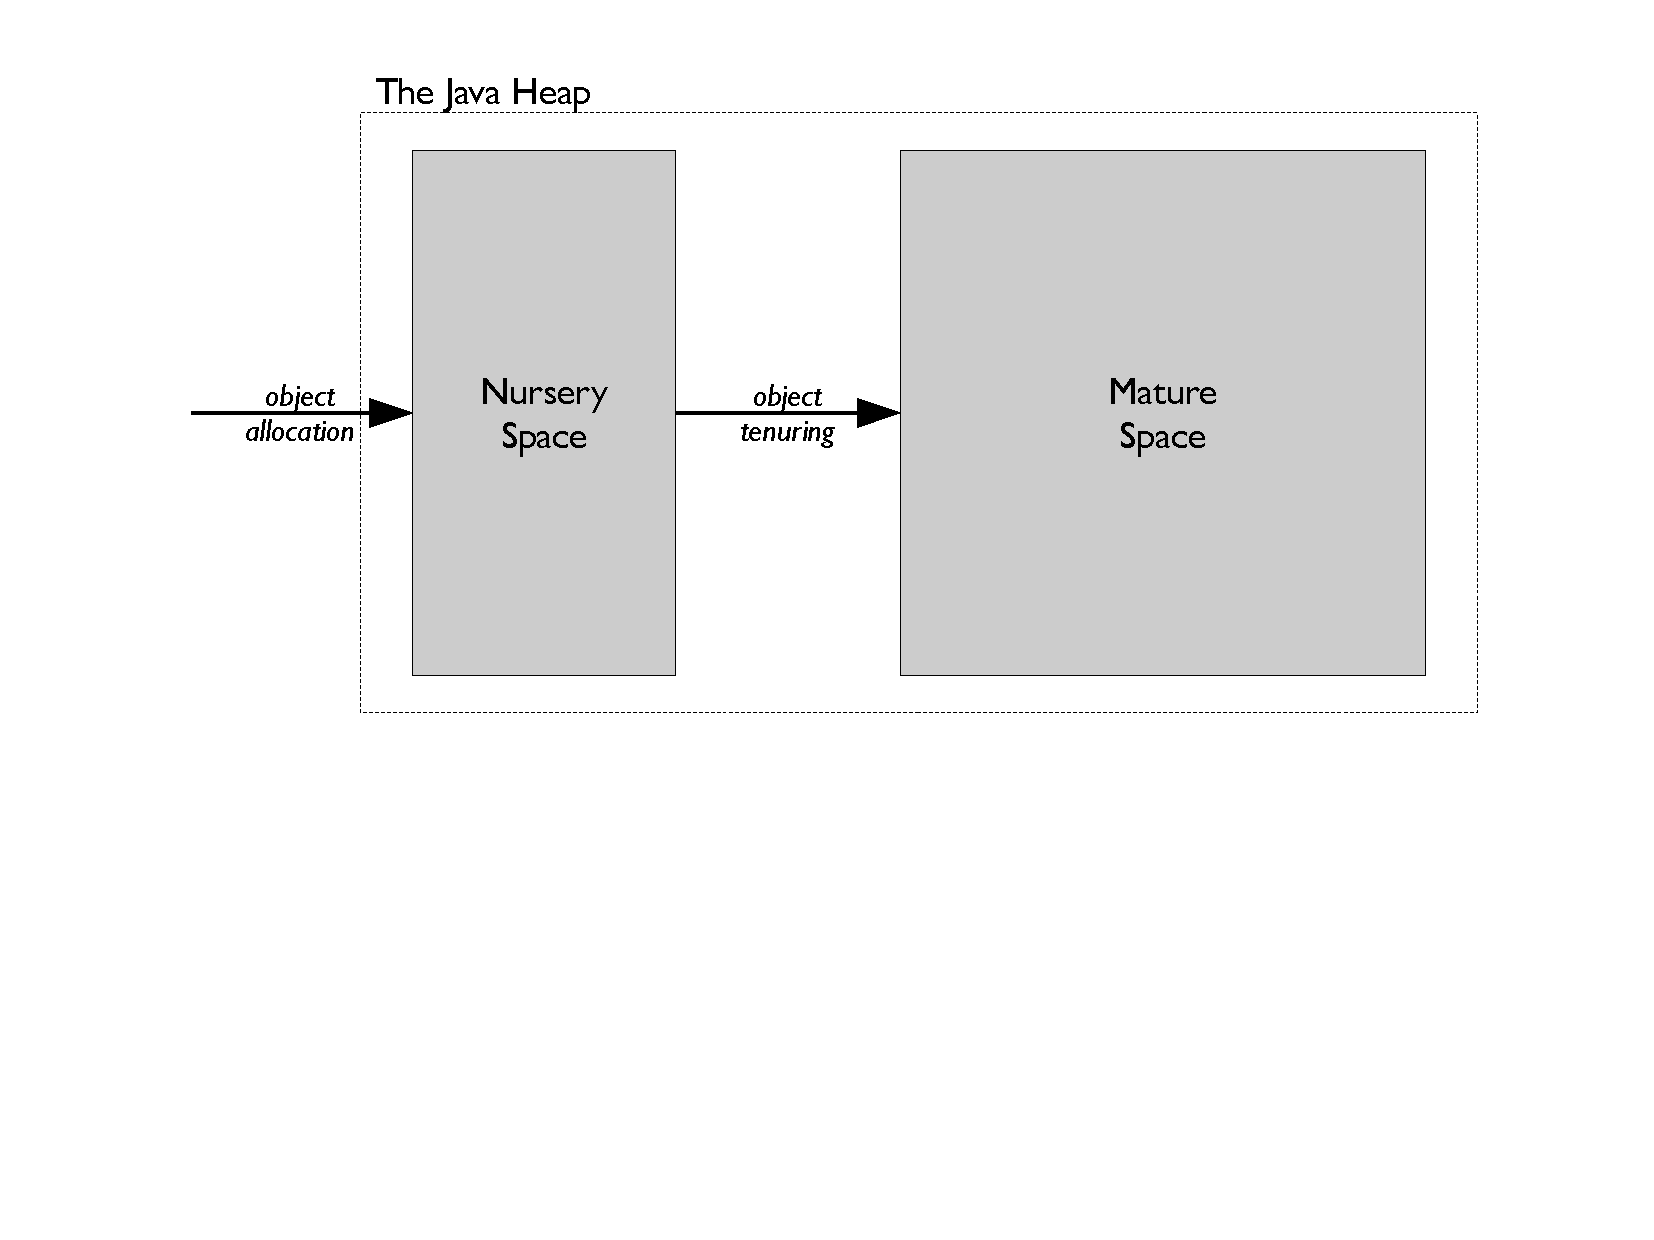
\includegraphics[width=0.6\textwidth]{part2/Figures/lifetime/nursery}
	\caption{Oftentimes, the Java heap is split into two sub-heaps. The nursery
	space stores newly-allocated objects, and the mature space stores objects that
	have been tenured. The garbage collector tenures an object after it
	survives a sufficient number of nursery garbage collections.}
	\label{fig:nursery-and-mature}
\end{figure}

To optimize for applications that create a large number of temporary objects,
some garbage collection strategies attempt to separate the short-lived and
long-lived objects into two separate heaps. These two heaps are typically called
the \emph{nursery} and \emph{mature} spaces, as illustrated in
\autoref{fig:nursery-and-mature}. The usual behavior is for objects to be
allocated in the nursery and, if they survive a sufficient number of garbage
collection cycles, to be \emph{tenured} to the mature space. If a large majority
of the objects in the nursery are no longer live at the time the \jre runs a
garbage collection on the nursery heap, then a traversal of the nursery help will
only touch a small number of memory pages. In this way, ignoring the costs of
initialization, reclaiming objects that are short-lived can be very cheap. Some
collectors allow you to specify a separate maxmum size for each, and some let you
specify only the maximum nursery size and the total maximum heap consumption (via
\code{-Xmx}.)

\paragraph{The Permspace Heap}
\index{Constant Pools}
\index{Permspace}
In addition to separating new and old objects, the \jre stores information about
classes in memory areas that are separate from those for instances of classes.
Some \jres create
a distinct heap for this data, one that can be sized like the other heaps.
Other \jres store this data in an undifferentiated part of the general native
heap. The Sun \jre is in the former camp, while the IBM and JRockit \jres are in
the latter camp.

In either case, the \jre needs to allocate memory
 in which to store data that is very unlikely to ever become
garbage. This includes the \jres metadata for your Java classes, along with the
executable code for your methods. In addition, any strings that you have
interned will be stored in this heap, along with any objects that the source
code compiler has decided to store in the \emph{constant pool} for a class;
these objects include any static strings, such as the one in this code snippet:

\begin{figure}
\centering
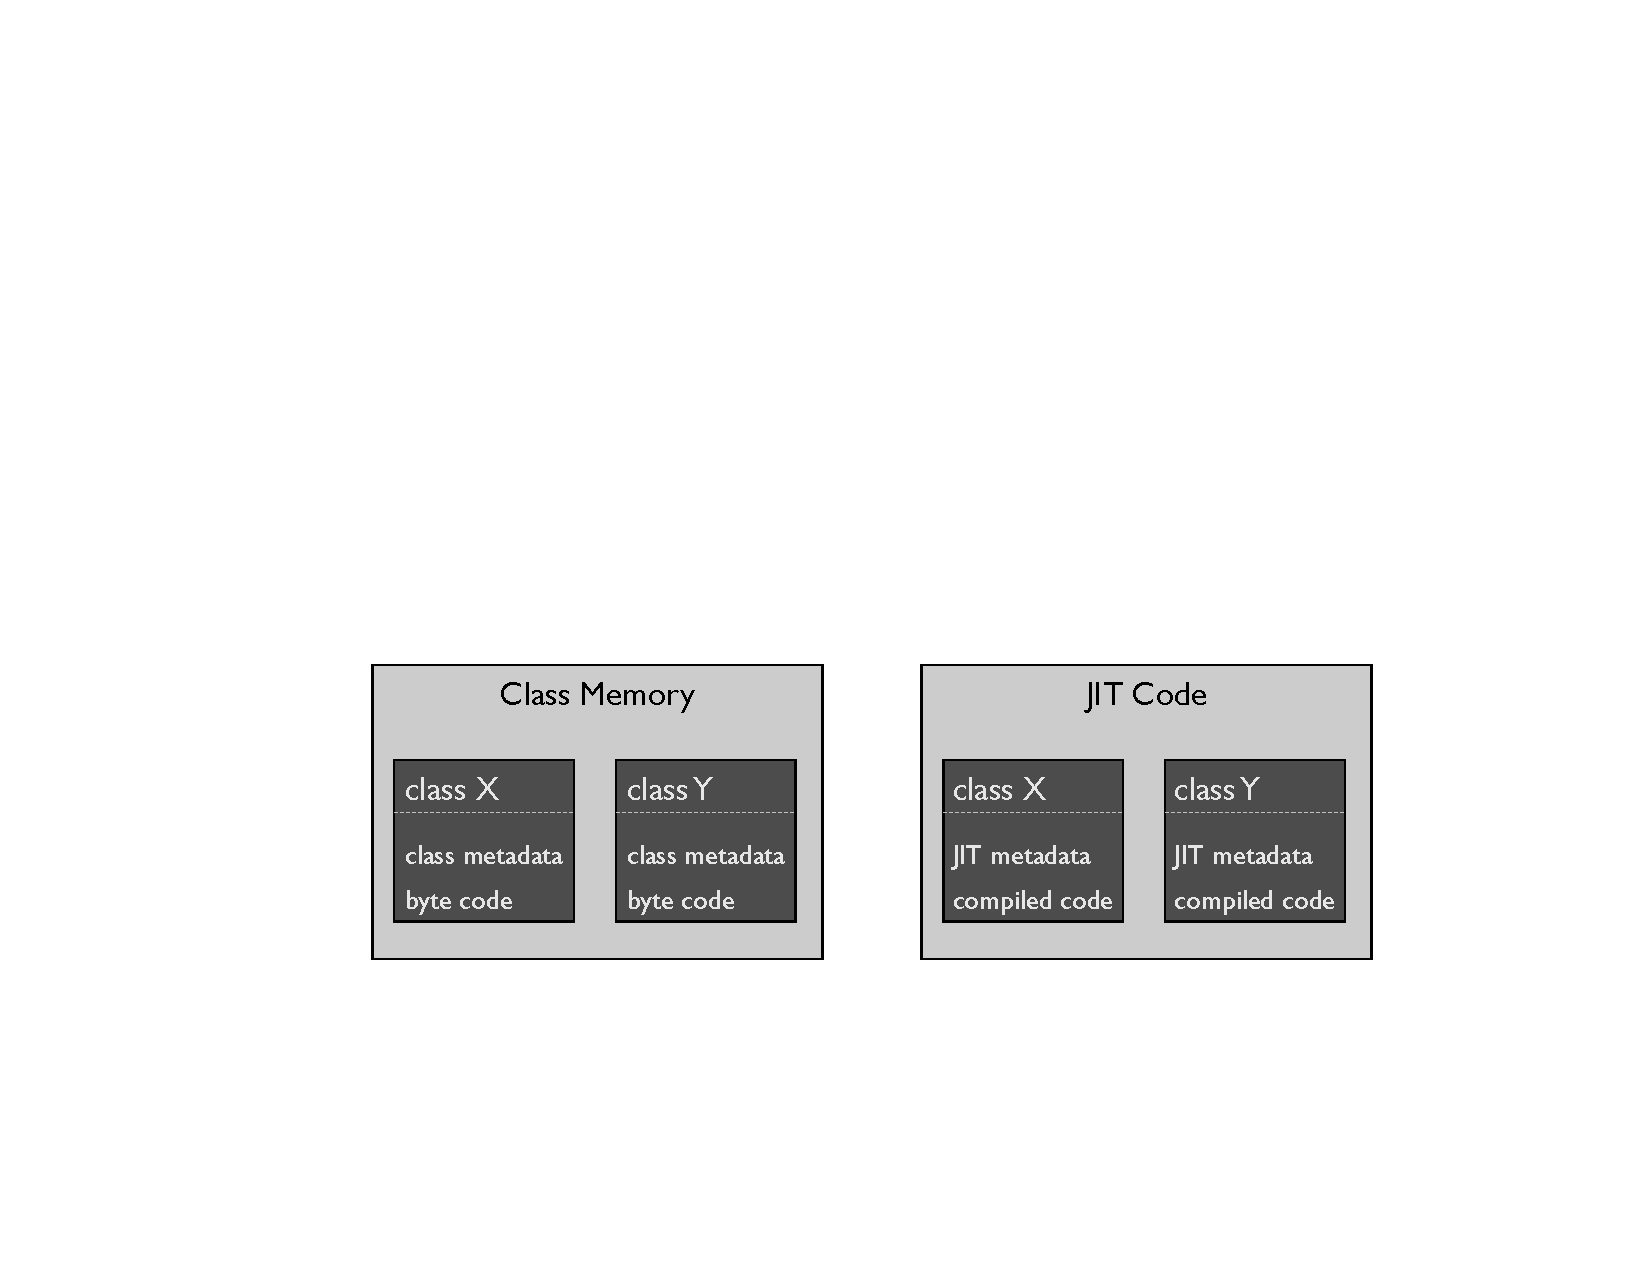
\includegraphics[width=0.75\textwidth]{part2/Figures/lifetime/heaps_and_stacks_classes}
\caption{The \jre also manages classes and compiled code, but in separate
	heaps. With some \jres, this data is combined into a single heap, called the
	\emph{Permspace} heap, which is sized via {\tt -XX:MaxPermSize}.}
\label{fig:heaps_and_stacks_classes}
\end{figure}


\begin{shortlisting}
System.out.println("aStaticString");
\end{shortlisting} 

The maximum size of Permspace, like the other heaps in Java, can often be
specified on the command line. In some cases, you may find that your application
requires a suspciously large maximum size for Permspace.
 
\begin{example}{Class Duplication and Excessive Permspace}
A Java Enterprise Edition (JEE) server application is deployed as 100 separate
applications, each in its own Web Application Archive (termed \code{war}) file.
Each \code{war} file contains duplicate class files for logic common to some, or even all applications.
The development team didn't think to worry about this, figuring that the
\jre would notice and remove the duplication. They were wrong, due to
requirements of the JEE specification, and suffered from excessive Permspace
consumption.

In JEE, each \code{war} file represents a distinct application, probably
separately developed. Having been coded separately, the JEE model assumes the
worst, that the applications will collide in their use of the static fields of
classes. Therefore, each \code{war} is loaded into a separate classloader, with
the result that the class duplication is not removed. The server application
required 500 megabytes for its Permspace heap, despite having under 100 megabytes
of distinct class data.
\end{example}


%% DO WE NEED THIS?
%\paragraph{Concurrent, Parallel, and Real-time Collection}
%\index{Concurrent GC}
%\index{Parallel GC}
%\index{Real-time GC}

\section{Building Your Own Lifetime Mechanisms}
\paragraph{The Reference Condundrum}

If you choose to leverage weak and soft references, you are in for a treat of
complex programming. There is a complex programming hassle that stems from
\class{WeakReference} and \class{SoftReference} being normal Java objects. If a
weak reference does not prevent an object from being reclaimable, and the weak
reference itself is represented by a Java object, then what is to keep the
\class{WeakReference} object itself from being reclaimed? The same thing holds
for soft references.

The only way to prevent a weak reference object from being immediately reclaimed
is to reference them, somehow, with strong references. If your goal is to
connect one object with another, via a weak or soft reference, then your job can be
straightforward. The above code, with \code{A.getB()}, works pretty well, as long
as it is properly modified to avoid the race condition. The only room for
improvement is unnecessary carrying around the \class{WeakReference} object
itself for the lifetime of the \class{A} instance, even after the weakly
referenced \class{B} has been reclaimed.

This baggage, of the reference wrappers, runs the risk of being a major
contributor to the overhead of using the weak or soft referencing mechanism. The
cost of a \class{SoftReference} wrapper is typically 12 bytes for the object
header, 4 bytes for the pointer to the referent, and 16 bytes for the clocks
necessary to implement an LRU eviction; it turns out that, to facilitate the
interaction with the JVM, every reference requires an extra 3 pointers, or 12
bytes, on top of these costs. In total, then, every soft reference you use in
your program costs at least 48 bytes. If the \class{A} object consumes only 24
bytes on its own, then softly referencing a \class{B} instance triples the unit
ost of \class{A}. A weak reference wrapper saves those 16 bytes of clocks, and
so costs a still high 32 bytes per wrapper.

The overhead grows even higher when you wish to associate a \class{B}
with an \class{A}, but cannot modify the class definition of \class{A}. In this case, you
must introduce a map in which to store the relation between the two. Worse,
however, is that this construct now leaks memory. When the \class{B} objects are
reclaimed, the map will still hold a strong reference to the reference object
that was serving as a wrapper around that reclaimed \class{B}.

\paragraph{The Basics of Reference Queue Management}
\index{Reference Queues}
\label{sec:reference-queue-basics}

Java provides \emph{reference queues} as a way to avoid this extra baggage, and
to avoid memory leaks in the use of weak and soft references. Using reference
queues adds an extra layer of complexity to an already difficult programming
task, but they are necessary for most uses of weak and soft references. You can
construct a reference wrapper with an associated reference queue. If you do so,
then the associated object, when the \jre decides to clip the weak or soft
reference, will not become immediately reclaimable. Instead, two special things
happen. First, the wrapper will be placed on the associated reference queue.
Second, once the wrapper is on the queue, the wrapper will change its behavior to
no longer reference the referent object. The latter effect complicates the clean
up process: the wrapper is placed on the queue, but calls to \code{get} no longer
return the referent object. 

The reference queue becomes a way for the \jre to notify you that it is ready to
clip the reference.  By associating a reference queue with weak and soft
references, you are given a cleanup hook.
% It is now up to you to finish the job.
With this hook, you can free up resources that are tied to the association that
the weak or soft references has established. For example, you have have native
resources tied to the association, such as open file descriptors. You can also
clean up the memory consumed by the reference objects themselves, such as by
assigning the \code{WeakReference<B> b} field to null in the example above. Since
any calls to \code{get}, from this hook, will return \code{null}, either your
hooks must not require access to the referent object, or you need to secure some
other means of accessing it.

One important task is cleaning up the reference queue itself. If you don't finish
the job properly, then the reference queue will become a source of memory leaks.
In order to detect that an object has been placed on the queue, your only
recourse is to call the \code{poll} method of the associated reference queue.
This will return the reference wrapper that is ready to be clipped, after
removing it from the queue. To avoid a memory leak in the reference queue, you
must call \code{poll} at least at the same rate at which you create reference
wrappers. That is, just before you create a reference wrapper, you must also poll
the reference queue, preferably in a loop, to see if any previously created
wrappers are ready to be clipped. This sounds complicated to get right, and it
is. Be careful!

If you are directly associating an \class{A} with a \class{B}, it is 
necessary to store the reference queue in a static field; storing it in an
instance field of \class{A} wouldn't make any sense. This means that the calls
to poll the reference queue must be protected with critical sections, in order
to avoid race conditions. However, this introduces lock contention problems:
\begin{shortlisting}
class A {
   static ReferenceQueue<B> refQueue;
   SoftReference<B> b;
   
   static void cleanupQueue() {
      synchronized(refQueue) {
         Reference<? extends B> bb;
         while ((bb = queue.poll()) != null) {
            // perform clean up bb
         }
      }
   }
   void makeB(B b) {
      cleanupQueue();   
      this.b = new SoftReference<B>(b, queue);
   }
}
\end{shortlisting}
\autoref{sec:lifetime-management-concurrency-issues} discusses solutions to this
concurrency problem.


\section{Implementing a Concurrent Cache}
\label{sec:lifetime-management-concurrency-issues}

If your program operates with many concurrent threads, you have to program
differently, because straightforward implementations of the above strategies will
result in concurrency issues. One of the primary problems will be lock
contention, as threads concurrently poll a reference queue. An important example
of this problem shows up in the implementation of a cache that can support many
concurrent users.\index{Caches, Concurrency Issues}

A cache is a map, usually of bounded size, with an eviction strategy for
maintaining that bound.\index{Caches} The Java standard library provides a
concurrent map implementation, in the form of the \class{ConcurrentHashMap}
class, but this is not a cache, because it has no eviction hooks with which one
can bound its size.

Following the soft reference rule, and using the basic guidelines for managing
reference queues from \autoref{sec:reference-queue-basics}, leads to a first
attempt at a \class{ConcurrentCache} implementation. You can extend the basic
concurrent hashmap, wrapping the map's values with soft references:
\begin{shortlisting}
class ConcurrentCache<K,V> extends ConcurrentHashMap<K,SoftReference<V>> {
   private final ReferenceQueue<V> refQueue = new ReferenceQueue<V>();
   
   protected void cleanupQueue() {
      SoftReference<V> v;
      while( (v = refQueue.poll()) != null) {
         remove(???); // oops!
      }
   }
}
\end{shortlisting}
Oops! This implementation provides no way to remove the key from the map, when
cleaning up the evicted entries. To fix this, you'll need to stash a pointer to
the key in the soft reference wrapper. It would be nice if the
\class{ConcurrentHashMap} implementation let you extend
its implementation so that its \class{\$Entry} class extended soft reference;
the \class{\$Entry} would serve this role perfectly. Instead, you have to
replicate this pointer structure, at a silly but unavoidable cost of memory
bloat. You can do so in a \class{CacheSoftReference} wrapper:
\begin{shortlisting}
class CacheSoftReference<K, V> extends SoftReference<V> {
   private final K k;
   
   public CacheSoftReference(K k, V v, ReferenceQueue<V> refQueue) {
      super(v, refQueue);
      this.k = k;
   }
}

class ConcurrentCache<K,V> extends ConcurrentHashMap<K,CacheSoftReference<K,V>> {
   private final ReferenceQueue<V> refQueue = new ReferenceQueue<V>();
   
   protected void cleanupQueue() {
      SoftReference<V> v;
      // poll causes lock contention!
      while( (v = refQueue.poll()) != null) {
         remove(v.k);
      }
   }
   
   public V put(K key, V value) {
      cleanupQueue();
      return super.put(key, new CacheSoftReference<K,V>(key,value,refQueue));
   }
   
   public V get(K key) {
      cleanupQueue();
      return super.get(key);
   }
}
\end{shortlisting}
This implementation still suffers from several critical problems. First, every
call to \code{put} must check the reference queue for pending evictions in order
to avoid unbounded growth of the eviction queue --- in the steady state,
\code{put} calls are likely to cause evictions. Even though \code{get} calls
won't cause evictions, in order to avoid pending evictions piling up as cached
elements are discovered to be unused, every call to \code{get} must also poll for
evictions. This can result in foiling the concurrency aspect of the
\class{ConcurrentHashMap}. Second, if the cache as a whole goes unused for a long
period of time, the pending evictions will pile up.

The only way to fix the lock contention problem, at least as of \javasix, is to
spawn a thread that periodically polls the reference queue for evicted entries.
This will also fix the second problem. This spawned thread's \code{run} method
will look just like the \code{cleanupQueue} method above, except that it should
loop indefinitely, and call \code{refQueue.remove()} rather than \code{poll()};
the former blocks until an eviction occurs (though you must still be careful to
check the return value for \code{null}, despite what the Javadocs claim).

At first sight, it would seem that you should be able to remove the calls to
\code{cleanupQueue} from the \code{put} and \code{get} methods. This, after all,
was the whole point of introducing the cleanup thread. However, this modified
implementation, while an improvement, suffers from a new problem. Now, if you
remove the \code{cleanupQueue} calls, when there is a large spike of \code{put}
calls in a short period of time, you are at risk of running out of Java heap due
to a large pileup of pending evictions.

You must have a safety valve in place to prevent this situation. One possibility
is to keep an approximate count of the number of \code{put} calls, and call
\code{cleanupQueue} only periodically. In order to avoid lock contention in
maintaining this count, you can do so in an unsynchronized way. There is still a
pathologic possibility that every racey increment of the put counter won't
actually increment the counter. If this worries you, you can use an
\class{AtomicInteger}, at increased expense. Instead of calling
\code{cleanupQueue} directly, the \code{put} method now calls a new
\code{helpCleaner} method:
\begin{shortlisting}
   static private final int SAFETY_VALVE = 1000;
   private void helpCleaner() {
      if (putCount.incrementAndGet() >= SAFETY_VALVE) {
         putCount.set(0);
         cleanupQueue();
      }
   }
\end{shortlisting}
There is no reason for \code{get} calls to call this method. The only point of
this safety valve is to avoid a sudden large influx of \code{put} calls. Indeed,
in this final implementation, the \code{ConcurrentCache} class needn't override
the \code{get} method of \code{ConcurrentHashMap}.

